\chapter{Climate Risk}

In what follow, we will focus on \textit{climate transition risk}. 
This refers to the financial risks that arise from the transition 
to a low-carbon economy. 

This includes risks from policy changes, technological innovations or 
market shifts. Transition risk can significantly 
affect the value of assets tied to carbon-intensive industries 
(brown assets) versus those aligned with a low-carbon economy (green assets).
Brown assets may face a decrease in value 
due to reduced demand or increased regulatory burden.
Green assets may benefit from increased demand and supportive 
policies during the transition.

As we have seen in the previous chapter, 
different states of the world represent different future 
scenarios. Climate transition introduces states 
like Current Policies (business-as-usual scenario) versus
Transition (low-carbon economy scenario). The pricing of assets 
should reflect their expected payoffs in these different states.

\begin{figure}[htbp]
    \centering
    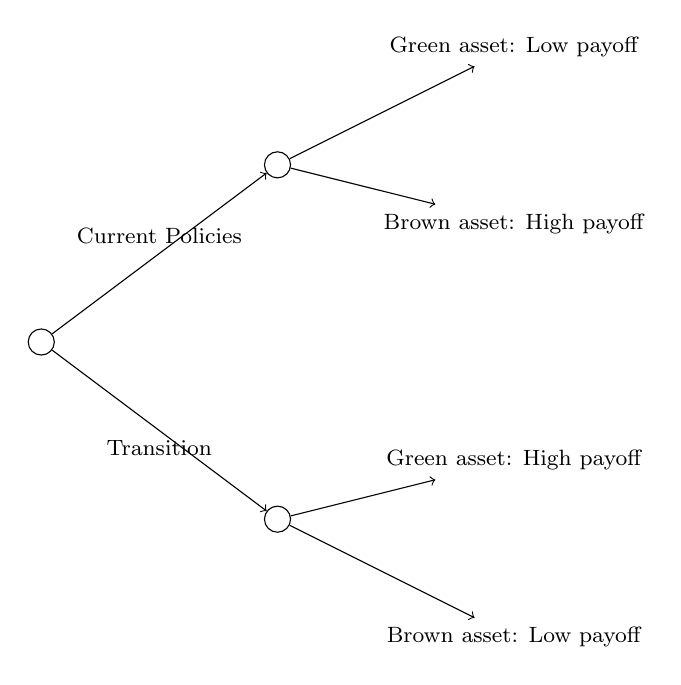
\begin{tikzpicture}[scale=1.5, every node/.style={font=\footnotesize}]

    % Nodes
    \node (start) at (0,0) [draw, circle] {};
    \node (current) at (2,1.5) [draw, circle] {};
    \node (transition) at (2,-1.5) [draw, circle] {};
    \node (current_green) at (4,2.5) {Green asset: Low payoff};
    \node (current_brown) at (4,1) {Brown asset: High payoff};
    \node (transition_green) at (4,-1) {Green asset: High payoff};
    \node (transition_brown) at (4,-2.5) {Brown asset: Low payoff};

    % Edges
    \draw[->] (start) -- (current) node[midway, above] {Current Policies};
    \draw[->] (start) -- (transition) node[midway, below] {Transition};
    \draw[->] (current) -- (current_green);
    \draw[->] (current) -- (current_brown);
    \draw[->] (transition) -- (transition_green);
    \draw[->] (transition) -- (transition_brown);
    
    % Labels

\end{tikzpicture}
    \caption{Climate States of the World}
    \label{fig:climate_risk}
\end{figure}

\section{Transition Scenarios as States of the World}

\section{What are Green and Brown Assets?}

\section{Expected Payoffs}

\section{Climate Risk Exposure and Expected Returns}